\scanpage{73}
\begin{tabular}{ll}
UNIVERSITE DES SCIENCES \& TECHNIQUES&Session de Juin 1978\\
\hspace*{2cm}DU LANGUEDOC&\\
\hspace*{2cm}\uline{Mathématiques}&
\end{tabular}

\begin{center}C4 Math. Pures et Approfondies,\\[12pt]
\uline{Option de M. Petrich}\end{center}

Décrire les classes de conjugaison de sous-groupes et d'éléments du groupe alterné $\unsure{G_5|\mathcal G_5}$, en indiquant leur interprétation géométrique en termes de l'icosaèdre.
\margin{-}
\figure{\begin{tikzpicture}\draw(0,0)--(1.3,0);\end{tikzpicture}}

\[
\zeta_A\in\Gamma(M_{0,I},L_A^*)
\]
\[
\prod_A\zeta_A\in\Gamma(M_{0,I},\bigotimes_A L_A)
\]
\figure{\begin{tikzpicture}\fill(0,0)circle(.035);\fill(.8,-.05)circle(.035);\fill(1.25,-.05)circle(.035);\end{tikzpicture}}
\deleted{$\unsure{\zeta}$}
\[
A\in\mathcal P_3(I)
\]
\figure{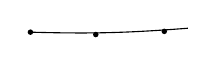
\begin{tikzpicture}\draw(0,0)to[bend right=3](2,0.05);\fill(0,0)circle(.035);\fill(.83,-.03)circle(.035);\fill(1.7,.01)circle(.035);\end{tikzpicture}}
\deleted{$\unsure{4|\ast}$}
\diagram{\begin{tikzcd}[ampersand replacement=\&]
M_{0,I}\arrow[r]\&M_{0 A}
\end{tikzcd}}
\margin{$i$}
\inserted{$\deleted{\unsure{2}}\ \frac{(n-1)(n-2)}{\deleted{\unsure{2}}\inserted{2}}=\nu$}
\[
\zeta=\prod\zeta_A\in L^{\otimes\deleted{\unsure{2\nu|4\nu}}}
\]
\[
L
\]
\diagram{\begin{tikzcd}[ampersand replacement=\&,column sep=large]
L_i\arrow[r,"{\varphi_{i,A,\omega}}"]\&\mathcal O
\end{tikzcd}}
\[
i\in A\in\mathcal P_3(I)
\]
\[
L=\deleted{\unsure{\prod}}\bigotimes_{i\in I}L_i
\]
\diagram{\begin{tikzcd}[ampersand replacement=\&,column sep=large]
L_i^2\arrow[r,no head,"{\psi_{i,A}}","\simeq"']\&\mathcal O
\end{tikzcd}}
\[
\nu=\frac{\unsure{(n-1)(n-1)|(n-1)(n-2)}}{\unsure{2}}
\]
\diagram{\begin{tikzcd}[ampersand replacement=\&,column sep=large]
\deleted{L_i}\arrow[r,no head,"{\deleted{\unsure{\varphi}}}","{\deleted{\simeq}}"']\&\deleted{\mathcal O}
\end{tikzcd}}
\[
\zeta\in L_i\qquad-\zeta
\]
\[
\zeta_{i,A}^{\deleted{\unsure{*}}}\in\Gamma L_i^2
\qquad\deleted{\unsure{L_2}}\qquad A
\]
\[
\zeta\in L_A^2\ \unsure{\sim}
\]
\figure{\begin{tikzpicture}\draw(0,0)to[out=-90,in=100](.05,-2.1)to[out=-80,in=140](.5,-2.7);\end{tikzpicture}}
\uline{Ex}\quad$n=4,\quad\nu=3$

on \unsure{trouve}\quad$L^{\otimes6}\simeq1$

\uline{Ex}\quad$n=5,\quad\nu=6,$\quad on \unsure{trouve}
\[
L^{\otimes\unsure{6|\sigma}}\simeq1
\]
\[
L_i\simeq L\otimes L_{\uline{I\setminus\{i\}}}^{-1}\simeq L\otimes p_i^*(\mathcal O(\unsure{1|{-1}}))
\]
\diagram{\begin{tikzcd}[ampersand replacement=\&,column sep=large]
p_i:\ M_{0,I}\arrow[r]\&M_{0,I\setminus\{i\}}\simeq\overline\Sigma
\end{tikzcd}}
\mspage{72}
